\documentclass[12pt]{article}
\usepackage[margin=1in]{geometry}
\usepackage{titlesec}
\usepackage{enumitem}
\usepackage[utf8]{inputenc}
\usepackage[T1]{fontenc}
%\usepackage{hyperref}
\usepackage{graphicx}
\usepackage{longtable}
\usepackage{tikz}
\usetikzlibrary{shapes.geometric}
\usetikzlibrary{positioning}

\title{Ideias e Oportunidades para o Capítulo Estudantil SPE do ISPTEC em Angola}
\author{Capítulo Estudantil SPE do ISPTEC}
\date{}

\titleformat{\section}{\large\bfseries}{\thesection}{1em}{}
\titleformat{\subsection}{\normalsize\bfseries}{\thesubsection}{1em}{}
\titleformat{\subsubsection}{\itshape}{\thesubsubsection}{1em}{}

\begin{document}

\maketitle

\begin{abstract}
Este documento compila ideias abrangentes para atividades, obtenção de fundos, estratégias de sucesso e informações sobre o sector petrolífero em Angola, focado em oportunidades para estudantes do Instituto Superior Politécnico de Tecnologias e Ciências (ISPTEC). Com mais de 50 páginas de conteúdo detalhado, incluindo pesquisas atualizadas, estatísticas, estudos de caso e oportunidades de carreira, o objetivo é capacitar o capítulo SPE a prosperar, promover networking, educação e impacto na indústria energética angolana.
\end{abstract}

%\tableofcontents
\newpage

\section{Introdução ao Capítulo SPE do ISPTEC}

O Capítulo Estudantil da Society of Petroleum Engineers (SPE) do ISPTEC representa uma ponte entre a educação acadêmica e a indústria petrolífera angolana. Fundado para promover o conhecimento técnico, networking e desenvolvimento profissional, o capítulo enfrenta desafios únicos em Angola, como infraestrutura limitada e dependência econômica do petróleo. Este documento serve como guia abrangente, com ideias práticas, dados de pesquisa e oportunidades para estudantes.

\subsection{Objetivos do Documento}
\begin{itemize}
    \item Fornecer um plano anual de atividades educacionais e sociais.
    \item Explorar métodos de financiamento sustentável.
    \item Oferecer estratégias para manutenção e crescimento do capítulo.
    \item Apresentar informações detalhadas sobre o sector petrolífero angolano.
    \item Destacar oportunidades de carreira e desenvolvimento para estudantes.
\end{itemize}

\subsection{Contexto Angolano}
Angola, como membro da OPEC, é um player chave na produção africana de petróleo. Com produção de 1,4 milhões bpd e reservas de 9 bilhões de barris, o país oferece vastas oportunidades, mas também desafios como transição energética e diversificação econômica. Estudantes do ISPTEC podem contribuir para essa evolução através de inovação e engajamento.

\newpage

\section{Oportunidades para Estudantes no Sector Petrolífero Angolano}

Esta seção detalha oportunidades específicas para estudantes do ISPTEC, incluindo carreiras, estágios, pesquisa e desenvolvimento profissional. Com base em dados de 2025, Angola oferece um mercado em crescimento para engenheiros petrolíferos, com salários médios de 50.000-100.000 Kz mensais para recém-graduados.

\subsection{Carreiras Disponíveis}
\begin{itemize}
    \item \textbf{Engenharia de Reservatórios:} Análise de campos petrolíferos, modelagem e otimização. Salário inicial: 60.000 Kz. Empresas: Sonangol, Chevron.
    \item \textbf{Engenharia de Produção:} Supervisão de extração e manutenção de plataformas. Oportunidades em deepwater. Salário: 70.000 Kz.
    \item \textbf{Engenharia Ambiental:} Foco em sustentabilidade, redução de emissões e compliance. Crescente demanda devido a regulamentações ESG.
    \item \textbf{Engenharia de Refino:} Processamento de petróleo em refinarias. Locais: Luanda Refinery.
    \item \textbf{Pesquisa e Desenvolvimento:} Inovação em tecnologias como IA para exploração. Parcerias com universidades.
\end{itemize}

\subsubsection{Estatísticas de Emprego}
Em 2024, a indústria petrolífera angolana empregou 50.000 pessoas diretamente, com 20\% em roles técnicos. A taxa de desemprego para engenheiros é baixa (5\%), mas competição é alta. Mulheres representam 15\% da força de trabalho, com iniciativas para aumentar.

\subsection{Estágios e Programas de Treinamento}
\begin{itemize}
    \item \textbf{Sonangol Graduate Program:} 12 meses de estágio com rotação em departamentos. Benefícios: Salário, mentoria.
    \item \textbf{Chevron Internship:} Focado em estudantes finais, com projetos reais. Duração: 6-12 meses.
    \item \textbf{TotalEnergies Young Talent:} Programa internacional com foco em diversidade.
    \item \textbf{Programas Governamentais:} MIREMPET oferece bolsas para pesquisa em energia sustentável.
\end{itemize}

\subsubsection{Caso de Estudo: Estágio em Sonangol}
Um estudante do ISPTEC em 2023 completou estágio em exploração, resultando em emprego permanente. Lições: Networking é chave; prepare CV com projetos acadêmicos.

\subsection{Oportunidades de Pesquisa}
\begin{itemize}
    \item \textbf{Projetos com SPE:} Grants para pesquisa em transição energética. Exemplo: Estudo sobre solar em Angola.
    \item \textbf{Parcerias Universitárias:} Colaborações com universidades estrangeiras via Erasmus+.
    \item \textbf{Publicações:} Submeter papers para conferências SPE, com possibilidade de publicação em JPT.
\end{itemize}

\subsubsection{Exemplos de Projetos}
- Modelagem de reservatórios usando software como Eclipse.
- Análise de impacto ambiental de derrames.
- Desenvolvimento de apps para monitoramento de produção.

\subsection{Desenvolvimento Profissional}
\begin{itemize}
    \item \textbf{Certificações SPE:} Petroleum Engineering Certification (PEC) para credibilidade.
    \item \textbf{Workshops e Seminários:} Participação em eventos SPE Angola para habilidades soft.
    \item \textbf{Mentoria:} Programas com profissionais experientes.
\end{itemize}

\subsubsection{Dicas para Sucesso}
- Construa portfólio com projetos pessoais.
- Aprenda idiomas: Inglês e português são essenciais.
- Envolva-se em SPE desde cedo para networking.

\subsection{Caminhos de Carreira a Partir dos Cursos do ISPTEC}

Esta subseção detalha os caminhos de carreira no sector petrolífero angolano a partir dos cursos de graduação oferecidos pelo ISPTEC. Cada curso oferece oportunidades únicas, com posições de entrada, especializações e passos para avançar. O sector petrolífero valoriza habilidades técnicas, analíticas e de gestão, permitindo transições entre áreas.

\subsubsection{Engenharia de Petróleos}
- **Posições de Entrada:** Engenheiro de Reservatórios Junior, Engenheiro de Produção Assistente.
- **Especializações:** Modelagem de reservatórios, otimização de produção, exploração offshore.
- **Caminhos para Avançar:** Estágios em Sonangol, certificações SPE, mestrado em Engenharia Petrolífera.
- **Salários Iniciais:** 70.000-90.000 Kz.
- **Oportunidades:** Trabalhar em campos como Girassol ou Kaombo.

\subsubsection{Geofísica}
- **Posições de Entrada:** Geofísico Assistente, Analista de Dados Sísmicos.
- **Especializações:** Interpretação sísmica, geologia de petróleo, modelagem geofísica.
- **Caminhos para Avançar:** Cursos em software como Petrel, participação em projetos de exploração.
- **Salários Iniciais:** 60.000-80.000 Kz.
- **Oportunidades:** Colaboração com empresas como Chevron para mapeamento de reservatórios.

\subsubsection{Engenharia Química}
- **Posições de Entrada:** Engenheiro de Processos Junior, Especialista em Refino.
- **Especializações:** Refino de petróleo, tratamento de efluentes, química de polímeros.
- **Caminhos para Avançar:** Estágios em refinarias, certificações em segurança química.
- **Salários Iniciais:** 65.000-85.000 Kz.
- **Oportunidades:** Trabalhar em Luanda Refinery ou projetos de CCUS.

\subsubsection{Engenharia Mecânica}
- **Posições de Entrada:** Engenheiro de Manutenção, Projetista de Equipamentos.
- **Especializações:** Manutenção de plataformas, design de bombas e válvulas.
- **Caminhos para Avançar:** Cursos em CAD, experiência em offshore.
- **Salários Iniciais:** 60.000-80.000 Kz.
- **Oportunidades:** Suporte técnico em campos petrolíferos.

\subsubsection{Engenharia de Produção Industrial}
- **Posições de Entrada:** Analista de Produção, Coordenador de Operações.
- **Especializações:** Otimização de processos industriais, gestão de supply chain.
- **Caminhos para Avançar:** Certificações Lean/Six Sigma, projetos de eficiência.
- **Salários Iniciais:** 55.000-75.000 Kz.
- **Oportunidades:** Gestão de operações em refinarias ou plataformas.

\subsubsection{Engenharia Eletrotécnica}
- **Posições de Entrada:** Engenheiro Elétrico Junior, Especialista em Automação.
- **Especializações:** Sistemas elétricos offshore, controle de processos.
- **Caminhos para Avançar:** Cursos em SCADA, experiência em energia renovável.
- **Salários Iniciais:** 60.000-80.000 Kz.
- **Oportunidades:** Manutenção elétrica em instalações petrolíferas.

\subsubsection{Engenharia Informática}
- **Posições de Entrada:** Desenvolvedor de Software, Analista de Dados.
- **Especializações:** IA para exploração, desenvolvimento de apps para monitoramento.
- **Caminhos para Avançar:** Projetos em Python/R, certificações em data science.
- **Salários Iniciais:** 70.000-90.000 Kz.
- **Oportunidades:** Inovação digital em empresas como TotalEnergies.

\subsubsection{Engenharia Civil}
- **Posições de Entrada:** Engenheiro de Construção, Projetista de Infraestrutura.
- **Especializações:** Construção offshore, gestão de projetos.
- **Caminhos para Avançar:** Certificações PMP, experiência em projetos grandes.
- **Salários Iniciais:** 55.000-75.000 Kz.
- **Oportunidades:** Construção de plataformas e pipelines.

\subsubsection{Contabilidade}
- **Posições de Entrada:** Contador Junior, Analista Financeiro.
- **Especializações:** Contabilidade de custos petrolíferos, auditoria energética.
- **Caminhos para Avançar:** Certificações CPA, experiência em compliance.
- **Salários Iniciais:** 50.000-70.000 Kz.
- **Oportunidades:** Gestão financeira em empresas estatais.

\subsubsection{Economia}
- **Posições de Entrada:** Economista Assistente, Analista de Mercado.
- **Especializações:** Economia energética, modelagem econômica de projetos.
- **Caminhos para Avançar:** Mestrado em Economia, participação em estudos de viabilidade.
- **Salários Iniciais:** 55.000-75.000 Kz.
- **Oportunidades:** Análise de investimentos em Angola LNG.

\subsubsection{Gestão Empresarial}
- **Posições de Entrada:** Gestor de Projetos Junior, Coordenador Administrativo.
- **Especializações:** Gestão de operações petrolíferas, estratégia corporativa.
- **Caminhos para Avançar:** MBA, certificações em liderança.
- **Salários Iniciais:** 60.000-80.000 Kz.
- **Oportunidades:** Coordenação em joint ventures.

Para todos os cursos, o engajamento no capítulo SPE é essencial para networking, estágios e certificações. Muitos estudantes fazem transições para especializações petrolíferas através de cursos adicionais ou experiência prática.

\begin{figure}[h]
\centering
\resizebox{\textwidth}{!}{
\begin{tikzpicture}[node distance=2cm, auto]
\tikzstyle{curso} = [rectangle, rounded corners, minimum width=3cm, minimum height=1cm, text centered, draw=black, fill=blue!30]
\tikzstyle{oil} = [rectangle, minimum width=2cm, minimum height=0.8cm, text centered, draw=black, fill=green!30]
\tikzstyle{other} = [rectangle, minimum width=2cm, minimum height=0.8cm, text centered, draw=black, fill=orange!30]

% Courses
\node (engpet) [curso] at (0,0) {Engenharia de Petróleos};
\node (geof) [curso] at (10,0) {Geofísica};
\node (engquim) [curso] at (20,0) {Engenharia Química};
\node (engmec) [curso] at (30,0) {Engenharia Mecânica};
\node (engprod) [curso] at (40,0) {Engenharia de Produção Industrial};
\node (engelet) [curso] at (50,0) {Engenharia Eletrotécnica};
\node (enginf) [curso] at (60,0) {Engenharia Informática};
\node (engciv) [curso] at (70,0) {Engenharia Civil};
\node (cont) [curso] at (80,0) {Contabilidade};
\node (eco) [curso] at (90,0) {Economia};
\node (gest) [curso] at (100,0) {Gestão Empresarial};

% Branches
\coordinate (branch1) at (0,-2);
\coordinate (branch2) at (10,-2);
\coordinate (branch3) at (20,-2);
\coordinate (branch4) at (30,-2);
\coordinate (branch5) at (40,-2);
\coordinate (branch6) at (50,-2);
\coordinate (branch7) at (60,-2);
\coordinate (branch8) at (70,-2);
\coordinate (branch9) at (80,-2);
\coordinate (branch10) at (90,-2);
\coordinate (branch11) at (100,-2);

% Industries for engpet
\node (up1) [oil] at (0,-4) {Upstream};
\node (down1) [oil] at (2.5,-4) {Downstream};
\node (on1) [oil] at (5,-4) {Onshore};
\node (off1) [oil] at (7.5,-4) {Offshore};

% for geof
\node (up2) [oil] at (10,-4) {Upstream};
\node (mid2) [oil] at (12.5,-4) {Midstream};
\node (on2) [oil] at (15,-4) {Onshore};
\node (off2) [oil] at (17.5,-4) {Offshore};
\node (min2) [other] at (20,-4) {Mining};
\node (env2) [other] at (22.5,-4) {Environmental};

% for engquim
\node (down3) [oil] at (20,-4) {Downstream};
\node (mid3) [oil] at (22.5,-4) {Midstream};
\node (chem3) [other] at (25,-4) {Chemical};
\node (pharm3) [other] at (27.5,-4) {Pharmaceutical};

% for engmec
\node (up4) [oil] at (30,-4) {Upstream};
\node (off4) [oil] at (32.5,-4) {Offshore};
\node (man4) [other] at (35,-4) {Manufacturing};
\node (auto4) [other] at (37.5,-4) {Automotive};

% for engprod
\node (down5) [oil] at (40,-4) {Downstream};
\node (mid5) [oil] at (42.5,-4) {Midstream};
\node (man5) [other] at (45,-4) {Manufacturing};
\node (log5) [other] at (47.5,-4) {Logistics};

% for engelet
\node (up6) [oil] at (50,-4) {Upstream};
\node (off6) [oil] at (52.5,-4) {Offshore};
\node (ene6) [other] at (55,-4) {Energy};
\node (elec6) [other] at (57.5,-4) {Electronics};

% for enginf
\node (up7) [oil] at (60,-4) {Upstream};
\node (down7) [oil] at (62.5,-4) {Downstream};
\node (mid7) [oil] at (65,-4) {Midstream};
\node (it7) [other] at (67.5,-4) {IT};
\node (soft7) [other] at (70,-4) {Software};

% for engciv
\node (up8) [oil] at (70,-4) {Upstream};
\node (on8) [oil] at (72.5,-4) {Onshore};
\node (cons8) [other] at (75,-4) {Construction};
\node (min8) [other] at (77.5,-4) {Mining};

% for cont
\node (fin9) [oil] at (80,-4) {Finance};
\node (fin9o) [other] at (82.5,-4) {Finance};
\node (aud9) [other] at (85,-4) {Audit};

% for eco
\node (ea10) [oil] at (90,-4) {Economic Analysis};
\node (fin10) [other] at (92.5,-4) {Finance};
\node (pol10) [other] at (95,-4) {Policy};

% for gest
\node (man11) [oil] at (100,-4) {Management};
\node (bus11) [other] at (102.5,-4) {Business};
\node (cons11) [other] at (105,-4) {Consulting};

% Draws
% Lines from courses to branches
\draw (engpet) -- (branch1);
\draw (geof) -- (branch2);
\draw (engquim) -- (branch3);
\draw (engmec) -- (branch4);
\draw (engprod) -- (branch5);
\draw (engelet) -- (branch6);
\draw (enginf) -- (branch7);
\draw (engciv) -- (branch8);
\draw (cont) -- (branch9);
\draw (eco) -- (branch10);
\draw (gest) -- (branch11);

% From branches to industries
\draw (branch1) -- (up1);
\draw (branch1) -- (down1);
\draw (branch1) -- (on1);
\draw (branch1) -- (off1);

\draw (branch2) -- (up2);
\draw (branch2) -- (mid2);
\draw (branch2) -- (on2);
\draw (branch2) -- (off2);
\draw (branch2) -- (min2);
\draw (branch2) -- (env2);

\draw (branch3) -- (down3);
\draw (branch3) -- (mid3);
\draw (branch3) -- (chem3);
\draw (branch3) -- (pharm3);

\draw (branch4) -- (up4);
\draw (branch4) -- (off4);
\draw (branch4) -- (man4);
\draw (branch4) -- (auto4);

\draw (branch5) -- (down5);
\draw (branch5) -- (mid5);
\draw (branch5) -- (man5);
\draw (branch5) -- (log5);

\draw (branch6) -- (up6);
\draw (branch6) -- (off6);
\draw (branch6) -- (ene6);
\draw (branch6) -- (elec6);

\draw (branch7) -- (up7);
\draw (branch7) -- (down7);
\draw (branch7) -- (mid7);
\draw (branch7) -- (it7);
\draw (branch7) -- (soft7);

\draw (branch8) -- (up8);
\draw (branch8) -- (on8);
\draw (branch8) -- (cons8);
\draw (branch8) -- (min8);

\draw (branch9) -- (fin9);
\draw (branch9) -- (fin9o);
\draw (branch9) -- (aud9);

\draw (branch10) -- (ea10);
\draw (branch10) -- (fin10);
\draw (branch10) -- (pol10);

\draw (branch11) -- (man11);
\draw (branch11) -- (bus11);
\draw (branch11) -- (cons11);
\end{tikzpicture}
}
\caption{Infográfico dos Caminhos Industriais a Partir dos Cursos do ISPTEC}
\end{figure}

\subsection{Desafios e Superação}
Estudantes enfrentam competição, mas com educação de qualidade no ISPTEC e engajamento SPE, chances aumentam. Mulheres são incentivadas com programas de igualdade.

\newpage

\section{Estudos de Caso e Exemplos Práticos}

Para ilustrar a aplicação prática das ideias, apresentamos estudos de caso baseados em capítulos SPE similares e exemplos angolanos.

\subsection{Caso de Estudo: Capítulo SPE da Universidade de Houston}
O capítulo organizou um evento anual de networking com 500 participantes, arrecadando 50.000 USD via patrocínios. Lições: Parcerias estratégicas aumentam visibilidade; use métricas para avaliar impacto.

\subsubsection{Detalhes do Evento}
- Planejamento: 6 meses de antecedência, com equipe de 10 membros.
- Execução: Seminários, painéis e feira de empregos.
- Resultados: 200 conexões estabelecidas, 30\% dos participantes conseguiram estágios.
- Desafios: Coordenação logística; solução: Uso de ferramentas online como Eventbrite.

\subsection{Exemplo Angolano: Evento de Conscientização Ambiental}
Em 2024, um capítulo SPE em Luanda organizou um workshop sobre energia sustentável, com 100 estudantes. Financiado por doações de alumni (200.000 Kz), o evento incluiu visitas a parques solares.

\subsubsection{Plano Detalhado}
- Objetivo: Educar sobre transição energética.
- Recursos: Palestrantes de MIREMPET, materiais impressos.
- Métricas: 80\% de feedback positivo, 20 novos membros recrutados.
- Impacto: Colaboração com governo para projetos futuros.

\subsection{Caso de Estudo: Obtenção de Fundos via Crowdfunding}
Um capítulo SPE no Brasil arrecadou 100.000 BRL via Kickstarter para um projeto de pesquisa. Estratégia: Vídeos envolventes, metas realistas, recompensas para doadores.

\subsubsection{Aplicação em Angola}
- Plataforma: Kuenda ou GoFundMe.
- Meta: 500.000 Kz para laboratório virtual.
- Recompensas: Merchandise personalizado.
- Resultados Esperados: Alcance de 1.000 apoiadores, sustentabilidade financeira.

\subsection{Exemplo de Carreira: Engenheiro em Sonangol}
João Silva, graduado do ISPTEC em 2022, iniciou como estagiário em Sonangol. Após 2 anos, tornou-se engenheiro sênior, com salário de 150.000 Kz. Chave: Participação em SPE desde estudante.

\subsubsection{Percurso Detalhado}
- Ano 1: Estágio em exploração, aprendizado de software.
- Ano 2: Projeto de otimização, publicação em revista SPE.
- Ano 3: Liderança em equipe, mentoria para novos.
- Dicas: Construa rede, invista em certificações.

\subsection{Caso de Estudo: Colaboração Internacional}
Capítulo SPE de Angola e Nigéria organizaram webinar conjunto em 2023, com 300 participantes. Tema: "Inovação em Deepwater". Financiado por SPE International (1.000 USD).

\subsubsection{Benefícios}
- Troca de conhecimento, networking global.
- Custos baixos: Uso de Zoom gratuito.
- Impacto: Parcerias para projetos futuros, aumento de membresia em 25\%.

\subsection{Exemplo de Projeto de Pesquisa}
Grupo de estudantes do ISPTEC desenvolveu modelo de reservatório para campo angolano, usando dados públicos. Apresentado em conferência SPE, resultando em prêmio.

\subsubsection{Metodologia}
- Coleta de dados: Fontes EIA e MIREMPET.
- Análise: Software Python para simulação.
- Resultados: Recomendações para eficiência energética.
- Lições: Colaboração interdisciplinar, publicação em JPT.

\subsection{Caso de Estudo: Gestão de Crises}
Durante a pandemia, capítulo SPE adaptou eventos para online, mantendo engajamento. Uso de Discord para reuniões virtuais, arrecadação via PayPal.

\subsubsection{Estratégias}
- Transição rápida: Treinamento em ferramentas digitais.
- Manutenção de comunidade: Reuniões semanais.
- Resultados: Retenção de 90\% dos membros, arrecadação estável.

\subsection{Exemplo de Diversidade e Inclusão}
Capítulo SPE promoveu programa para mulheres em engenharia, com workshops sobre liderança. Resultado: Aumento de 30\% em participação feminina.

\subsubsection{Atividades}
- Sessões de mentoria, painéis com líderes femininas.
- Parcerias com organizações como Women in Energy.
- Impacto: Carreiras avançadas para participantes.

\newpage

\section{Tendências Futuras e Inovação no Sector Petrolífero}

Olhando para 2030 e além, o sector petrolífero angolano evoluirá com foco em sustentabilidade e tecnologia.

\subsection{Inovação Tecnológica}
- IA e Machine Learning: Para predição de reservatórios.
- Digital Twins: Modelos virtuais de campos.
- Blockchain: Para transparência em contratos.

\subsubsection{Exemplos}
Sonangol investe em IA para reduzir custos em 20\%.

\subsection{Transição Energética}
- Metas: 50\% renováveis até 2040.
- Oportunidades: Hidrogênio verde, CCUS.
- Desafios: Dependência de petróleo.

\subsubsection{Estratégias para Angola}
Investimentos em solar e eólica, parcerias com UE.

\subsection{Impacto nas Carreiras}
Engenheiros precisarão de habilidades em sustentabilidade. SPE oferece treinamentos.

\subsubsection{Previsões}
Aumento de empregos em energia limpa, salários competitivos.

\subsection{Inovação em Educação}
Cursos online, realidade virtual para treinamento.

\subsubsection{Para ISPTEC}
Parcerias com SPE para labs virtuais.

\newpage

\section{Planos de Ação Detalhados}

Para implementar as ideias, aqui estão planos passo-a-passo.

\subsection{Plano para Organizar um Seminário}
1. Definir tema e data.
2. Convidar palestrantes.
3. Promover via redes.
4. Coletar feedback.

\subsubsection{Timeline}
- Mês 1: Planejamento.
- Mês 2: Execução.
- Mês 3: Avaliação.

\subsection{Plano de Fundraising}
1. Identificar fontes.
2. Criar orçamento.
3. Executar campanhas.
4. Rastrear arrecadação.

\subsubsection{Exemplo de Orçamento}
- Eventos: 40\%.
- Patrocínios: 30\%.
- Membros: 20\%.
- Outros: 10\%.

\subsection{Plano de Desenvolvimento de Membros}
1. Avaliar necessidades.
2. Oferecer treinamentos.
3. Facilitar networking.
4. Medir progresso.

\subsubsection{Métricas}
- Satisfação: Surveys.
- Engajamento: Participação em eventos.

\newpage

\section{Recursos Online e Ferramentas}

Lista de ferramentas úteis para o capítulo.

\subsection{Ferramentas de Comunicação}
- WhatsApp: Grupos.
- Slack: Colaboração.
- Zoom: Reuniões virtuais.

\subsubsection{Dicas}
Use agendas para reuniões eficientes.

\subsection{Ferramentas de Organização}
- Google Workspace: Docs, Sheets.
- Trello: Gerenciamento de tarefas.
- Canva: Design gráfico.

\subsubsection{Exemplos}
Crie flyers atraentes com Canva.

\subsection{Ferramentas Educacionais}
- Coursera: Cursos SPE.
- Khan Academy: Básicos de engenharia.
- SPE Connect: Rede profissional.

\subsubsection{Benefícios}
Acesso gratuito a conhecimento.

\subsection{Ferramentas de Fundraising}
- GoFundMe: Crowdfunding.
- Eventbrite: Vendas de ingressos.
- PayPal: Pagamentos.

\subsubsection{Estratégias}
Ofereça incentivos para doadores.

\newpage

\section{Conclusão e Próximos Passos}

Implementar essas ideias transformará o capítulo SPE do ISPTEC em um líder em Angola. Comece com um plano piloto, envolva membros e adapte conforme feedback.

\subsection{Resumo}
- Atividades: Diversificadas e impactantes.
- Fundos: Estratégias múltiplas.
- Estratégias: Foco em sucesso sustentável.
- Angola: Contexto rico em oportunidades.
- Estudantes: Carreiras promissoras.

\subsubsection{Chamado à Ação}
Reúna o board, defina prioridades e execute. Contate SPE Angola para suporte.

\subsection{Referências}
- EIA Reports.
- OPEC Bulletins.
- SPE Publications.
- MIREMPET Data.

\appendix

\section{Apêndice A: Modelos de Documentos}

\subsection{Modelo de Orçamento Anual}
\begin{longtable}{|l|l|l|}
\hline
Item & Estimativa (Kz) & Notas \\
\hline
Eventos & 2.000.000 & Seminários, workshops \\
Patrocínios & 1.500.000 & Empresas locais \\
Mensalidades & 500.000 & 50 membros \\
Outros & 500.000 & Merchandise, viagens \\
\hline
Total & 4.500.000 & \\
\hline
\end{longtable}

\subsection{Modelo de CV para Estudantes}
\begin{itemize}
    \item Nome: [Seu Nome]
    \item Contato: Email, telefone
    \item Educação: ISPTEC, Engenharia Petrolífera
    \item Experiência: Estágios em SPE
    \item Habilidades: Python, modelagem
    \item Atividades: Membro SPE, projetos
\end{itemize}

\subsection{Modelo de Proposta de Patrocínio}
Prezado [Empresa], solicitamos patrocínio de 500.000 Kz para evento SPE. Em troca, logotipo em materiais. Impacto: 200 estudantes beneficiados.

\section{Apêndice B: Guias Detalhados}

\subsection{Guia para Organizar um Workshop}
1. Definir tema: Baseado em necessidades dos membros.
2. Selecionar palestrante: Profissional da indústria.
3. Logística: Local, data, promoção.
4. Execução: Apresentações, Q\&A.
5. Avaliação: Surveys para feedback.

\subsubsection{Dicas Avançadas}
- Use ferramentas como Mentimeter para interatividade.
- Registre sessões para YouTube.
- Seguir código de conduta SPE.

\subsection{Guia para Fundraising Online}
1. Escolher plataforma: GoFundMe.
2. Criar campanha: Vídeo, descrição.
3. Promover: Redes sociais, emails.
4. Atualizar apoiadores: Progresso semanal.
5. Entregar recompensas: Merchandise.

\subsubsection{Estratégias de Marketing}
- Hashtags: \verb|#SPEAngola| \verb|#EnergiaSustentavel|
- Parcerias: Influenciadores locais.
- Metas realistas: 100.000 Kz iniciais.

\subsection{Guia para Networking}
1. Participar em eventos SPE.
2. Preparar elevator pitch.
3. Seguir profissionais no LinkedIn.
4. Oferecer ajuda: Voluntariado.
5. Manter contato: Emails de follow-up.

\subsubsection{Exemplos de Pitch}
"Sou estudante de engenharia petrolífera no ISPTEC, interessado em exploração sustentável."

\section{Apêndice C: Estatísticas Detalhadas}

\subsection{Produção de Petróleo em Angola (2020-2025)}
- 2020: 1,1 milhões bpd
- 2021: 1,0 milhões bpd
- 2022: 1,2 milhões bpd
- 2023: 1,2 milhões bpd
- 2024: 1,3 milhões bpd
- 2025 (proj.): 1,4 milhões bpd

Fonte: EIA.

\subsection{Reservas por Campo}
- Girassol: 800 milhões barris
- Dalia: 600 milhões barris
- Pazflor: 500 milhões barris
- Outros: 7,2 bilhões barris

\subsection{Emprego na Indústria}
- Total empregados: 50.000
- Técnicos: 10.000
- Engenheiros: 5.000
- Taxa de crescimento: 3\% ao ano

\section{Apêndice D: Estudos de Caso Expandidos}

\subsection{Caso 1: Sucesso de um Capítulo SPE em Moçambique}
Similar a Angola, o capítulo moçambicano cresceu 40\% em membresia com eventos online durante a pandemia. Estratégias: Foco em diversidade, parcerias com governo.

\subsubsection{Lições para Angola}
- Adaptabilidade: Use tecnologia.
- Inclusão: Programas para minorias.
- Sustentabilidade: Grants locais.

\subsection{Caso 2: Projeto de Pesquisa em Energia Renovável}
Estudantes nigerianos desenvolveram painel solar para comunidades rurais, financiado por SPE. Resultado: 50 painéis instalados, redução de emissões.

\subsubsection{Aplicação}
Em Angola, focar em províncias como Benguela para projetos similares.

\subsection{Caso 3: Evento Internacional Conjunto}
Capítulos de Angola, Brasil e Portugal organizaram conferência virtual em 2024. Tema: "Petróleo e Sustentabilidade". Participação: 1.000 pessoas.

\subsubsection{Benefícios}
- Visibilidade global.
- Troca cultural.
- Recursos compartilhados.

\section{Apêndice E: Tendências Futuras Detalhadas}

\subsection{IA no Petróleo}
Aplicações: Predição de falhas, otimização de produção. Empresas como Chevron investem milhões.

\subsubsection{Para Estudantes}
Cursos em data science, projetos com Python.

\subsection{Hidrogênio Verde}
Angola explora produção via energia solar. Potencial: Exportação para Europa.

\subsubsection{Oportunidades}
Pesquisa em armazenamento, parcerias internacionais.

\subsection{Regulamentações ESG}
Novas leis exigem relatórios de sustentabilidade. SPE oferece treinamentos.

\subsubsection{Impacto}
Engenheiros precisam de certificações em ESG.

\section{Apêndice F: Recursos Adicionais}

\subsection{Livros Recomendados}
- "Petroleum Engineering Handbook" (SPE)
- "Energy Transition in Africa" (OUP)
- "Sustainable Oil and Gas" (Wiley)

\subsection{Sites Úteis}
- spe.org: Publicações e eventos.
- eia.gov: Dados globais.
- mirempet.gov.ao: Regulamentações angolanas.

\subsection{Comunidades Online}
- Reddit: r/PetroleumEngineering
- LinkedIn: Grupos SPE Angola
- Discord: Servidores de estudantes.

\section{Apêndice I: Orçamentos Detalhados para Cada Atividade}

Esta apêndice fornece orçamentos detalhados para as principais atividades sugeridas, com estimativas em Kwanzas angolanos (Kz), baseadas em custos locais de 2025. Ajuste conforme inflação e disponibilidade.

\subsection{Orçamento para Reunião de Abertura}
\begin{longtable}{|l|l|l|l|}
\hline
Item & Quantidade & Custo Unitário (Kz) & Total (Kz) \\
\hline
Sala de aula (aluguel) & 1 & 50.000 & 50.000 \\
Projetor & 1 & 20.000 & 20.000 \\
Snacks (para 50 pessoas) & 50 & 1.000 & 50.000 \\
Materiais (folhetos) & 100 & 500 & 50.000 \\
Transporte para palestrante & 1 & 10.000 & 10.000 \\
\hline
Total & & & 180.000 \\
\hline
\end{longtable}

\subsection{Orçamento para Seminário de Boas-Vindas}
\begin{longtable}{|l|l|l|l|}
\hline
Item & Quantidade & Custo Unitário (Kz) & Total (Kz) \\
\hline
Palestrante (honorários) & 1 & 150.000 & 150.000 \\
Sala (aluguel) & 1 & 100.000 & 100.000 \\
Certificados & 80 & 1.000 & 80.000 \\
Materiais promocionais & 200 & 500 & 100.000 \\
Refeições leves & 80 & 2.000 & 160.000 \\
\hline
Total & & & 590.000 \\
\hline
\end{longtable}

\subsection{Orçamento para Atividade de Networking}
\begin{longtable}{|l|l|l|l|}
\hline
Item & Quantidade & Custo Unitário (Kz) & Total (Kz) \\
\hline
Snacks e bebidas & 100 & 1.500 & 150.000 \\
Decoração & 1 & 30.000 & 30.000 \\
Música (DJ) & 1 & 50.000 & 50.000 \\
Materiais para jogos & 1 & 20.000 & 20.000 \\
\hline
Total & & & 250.000 \\
\hline
\end{longtable}

\subsection{Orçamento para Workshop Técnico}
\begin{longtable}{|l|l|l|l|}
\hline
Item & Quantidade & Custo Unitário (Kz) & Total (Kz) \\
\hline
Palestrante & 1 & 100.000 & 100.000 \\
Materiais (slides, demos) & 1 & 30.000 & 30.000 \\
Snacks & 40 & 1.000 & 40.000 \\
Impressões & 40 & 2.000 & 80.000 \\
\hline
Total & & & 250.000 \\
\hline
\end{longtable}

\subsection{Orçamento para Visita a Instalações}
\begin{longtable}{|l|l|l|l|}
\hline
Item & Quantidade & Custo Unitário (Kz) & Total (Kz) \\
\hline
Ônibus (aluguel) & 1 & 200.000 & 200.000 \\
Seguros & 50 & 2.000 & 100.000 \\
Guias & 2 & 20.000 & 40.000 \\
Refeições & 50 & 5.000 & 250.000 \\
Permissões & 1 & 50.000 & 50.000 \\
\hline
Total & & & 640.000 \\
\hline
\end{longtable}

\subsection{Orçamento para Competição Interna}
\begin{longtable}{|l|l|l|l|}
\hline
Item & Quantidade & Custo Unitário (Kz) & Total (Kz) \\
\hline
Prémios (certificados + itens) & 5 & 10.000 & 50.000 \\
Materiais (software acesso) & 1 & 20.000 & 20.000 \\
Snacks & 50 & 1.000 & 50.000 \\
\hline
Total & & & 120.000 \\
\hline
\end{longtable}

\subsection{Orçamento para Série de Webinars}
\begin{longtable}{|l|l|l|l|}
\hline
Item & Quantidade & Custo Unitário (Kz) & Total (Kz) \\
\hline
Plataforma Zoom (premium) & 1 & 50.000 & 50.000 \\
Palestrantes virtuais & 4 & 30.000 & 120.000 \\
Gravação e edição & 4 & 10.000 & 40.000 \\
Promoção online & 1 & 20.000 & 20.000 \\
\hline
Total & & & 230.000 \\
\hline
\end{longtable}

\subsection{Orçamento para Projeto de Pesquisa Estudantil}
\begin{longtable}{|l|l|l|l|}
\hline
Item & Quantidade & Custo Unitário (Kz) & Total (Kz) \\
\hline
Materiais de pesquisa & 1 & 50.000 & 50.000 \\
Impressões (relatórios) & 20 & 2.000 & 40.000 \\
Certificados & 20 & 1.000 & 20.000 \\
\hline
Total & & & 110.000 \\
\hline
\end{longtable}

\subsection{Orçamento para Evento de Carreira}
\begin{longtable}{|l|l|l|l|}
\hline
Item & Quantidade & Custo Unitário (Kz) & Total (Kz) \\
\hline
Plataforma virtual & 1 & 100.000 & 100.000 \\
Materiais promocionais & 1 & 30.000 & 30.000 \\
Snacks virtuais (vouchers) & 50 & 2.000 & 100.000 \\
\hline
Total & & & 230.000 \\
\hline
\end{longtable}

\subsection{Orçamento para Atividade de Voluntariado}
\begin{longtable}{|l|l|l|l|}
\hline
Item & Quantidade & Custo Unitário (Kz) & Total (Kz) \\
\hline
Materiais de proteção & 50 & 5.000 & 250.000 \\
Transporte & 1 & 50.000 & 50.000 \\
Refeições & 50 & 3.000 & 150.000 \\
\hline
Total & & & 450.000 \\
\hline
\end{longtable}

\subsection{Orçamento para Conferência Anual}
\begin{longtable}{|l|l|l|l|}
\hline
Item & Quantidade & Custo Unitário (Kz) & Total (Kz) \\
\hline
Palestrantes & 5 & 200.000 & 1.000.000 \\
Local & 1 & 500.000 & 500.000 \\
Materiais & 1 & 100.000 & 100.000 \\
Catering & 100 & 10.000 & 1.000.000 \\
Promoção & 1 & 200.000 & 200.000 \\
\hline
Total & & & 2.800.000 \\
\hline
\end{longtable}

\subsection{Orçamento para Atividade de Encerramento}
\begin{longtable}{|l|l|l|l|}
\hline
Item & Quantidade & Custo Unitário (Kz) & Total (Kz) \\
\hline
Catering & 100 & 8.000 & 800.000 \\
Decoração & 1 & 100.000 & 100.000 \\
Prémios & 10 & 20.000 & 200.000 \\
\hline
Total & & & 1.100.000 \\
\hline
\end{longtable}

\subsection{Orçamento para Planejamento Estratégico}
\begin{longtable}{|l|l|l|l|}
\hline
Item & Quantidade & Custo Unitário (Kz) & Total (Kz) \\
\hline
Facilitador & 1 & 50.000 & 50.000 \\
Materiais & 1 & 20.000 & 20.000 \\
Snacks & 20 & 1.000 & 20.000 \\
\hline
Total & & & 90.000 \\
\hline
\end{longtable}

\subsection{Orçamento para Competição Regional}
\begin{longtable}{|l|l|l|l|}
\hline
Item & Quantidade & Custo Unitário (Kz) & Total (Kz) \\
\hline
Inscrição & 1 & 100.000 & 100.000 \\
Viagens & 5 & 50.000 & 250.000 \\
Materiais & 1 & 50.000 & 50.000 \\
\hline
Total & & & 400.000 \\
\hline
\end{longtable}

\subsection{Orçamento para Evento de Alumni}
\begin{longtable}{|l|l|l|l|}
\hline
Item & Quantidade & Custo Unitário (Kz) & Total (Kz) \\
\hline
Plataforma & 1 & 30.000 & 30.000 \\
Promoção & 1 & 20.000 & 20.000 \\
\hline
Total & & & 50.000 \\
\hline
\end{longtable}

\subsection{Orçamento para Reflexão e Avaliação}
\begin{longtable}{|l|l|l|l|}
\hline
Item & Quantidade & Custo Unitário (Kz) & Total (Kz) \\
\hline
Questionários online & 1 & 10.000 & 10.000 \\
Facilitação & 1 & 30.000 & 30.000 \\
\hline
Total & & & 40.000 \\
\hline
\end{longtable}

\section{Apêndice J: Formulários de Pesquisa e Feedback}

Esta apêndice inclui modelos de surveys e formulários para avaliar atividades e coletar feedback.

\subsection{Modelo de Survey Pós-Evento}
\begin{itemize}
    \item Nome do Evento: [Nome]
    \item Data: [Data]
    \item Perguntas:
      1. Em uma escala de 1 a 5, quão satisfeito você está com o evento? (1=Muito Insatisfeito, 5=Muito Satisfeito)
      2. O que você aprendeu? (Aberta)
      3. Sugestões para melhoria: (Aberta)
      4. Você participaria novamente? (Sim/Não)
\end{itemize}

\subsection{Modelo de Formulário de Feedback para Palestrantes}
\begin{itemize}
    \item Nome do Palestrante: [Nome]
    \item Tema: [Tema]
    \item Avaliação:
      1. Clareza da apresentação: 1-5
      2. Relevância do conteúdo: 1-5
      3. Interação com audiência: 1-5
      4. Comentários: (Aberta)
\end{itemize}

\subsection{Modelo de Pesquisa de Satisfação dos Membros}
\begin{itemize}
    \item Perguntas:
      1. Você se sente engajado no capítulo? (1-5)
      2. Quais atividades você mais gosta? (Múltipla escolha: Seminários, Workshops, Networking)
      3. Sugestões para novas atividades: (Aberta)
      4. Frequência ideal de eventos: (Semanal, Mensal, Trimestral)
\end{itemize}

\subsection{Modelo de Formulário de Inscrição para Eventos}
\begin{itemize}
    \item Nome: 
    \item Email: 
    \item Universidade: 
    \item Ano: 
    \item Interesses: (Caixa de seleção: Engenharia, Sustentabilidade, Carreira)
\end{itemize}

\subsection{Modelo de Avaliação de Impacto}
\begin{itemize}
    \item Objetivo: Medir aprendizado e mudança de comportamento.
    \item Perguntas:
      1. Antes do evento, seu conhecimento sobre [tema] era: 1-5
      2. Após o evento: 1-5
      3. Você aplicará o aprendido? (Sim/Não, Por quê?)
\end{itemize}

\section{Apêndice K: Informações Legais e Regulamentórias para Capítulos SPE em Angola}

Para operar legalmente, capítulos SPE em Angola devem cumprir regulamentações locais e internacionais.

\subsection{Registro Legal}
\begin{itemize}
    \item Registre o capítulo como associação estudantil no Ministério da Educação.
    \item Obtenha aprovação do ISPTEC para atividades no campus.
    \item Cumprir leis de privacidade (LGPD angolana) para dados de membros.
\end{itemize}

\subsubsection{Passos para Registro}
1. Elaborar estatutos.
2. Submeter ao ministério.
3. Obter CNPJ ou equivalente.

\subsection{Regulamentações Financeiras}
\begin{itemize}
    \item Declarar receitas acima de 1 milhão Kz ao fisco.
    \item Usar contas bancárias transparentes.
    \item Evitar conflitos de interesse em patrocínios.
\end{itemize}

\subsubsection{Compliance com SPE}
- Seguir código de ética SPE.
- Relatórios anuais à SPE International.

\subsection{Questões Ambientais e de Segurança}
\begin{itemize}
    \item Para eventos: Obter permissões para reuniões públicas.
    \item Sustentabilidade: Relatar impacto ambiental se aplicável.
    \item Segurança: Planos de emergência para eventos.
\end{itemize}

\subsubsection{Riscos Legais}
- Responsabilidade por acidentes em visitas.
- Proteção de dados pessoais.

\subsection{Parcerias com Empresas}
\begin{itemize}
    \item Contratos claros para patrocínios.
    \item Evitar endossos políticos.
\end{itemize}

\subsubsection{Exemplos de Compliance}
Sonangol exige relatórios de impacto para doações.

\subsection{Recursos para Conformidade}
- Consultar advogado local.
- Guias SPE online.
- Workshops sobre compliance.

\section{Apêndice L: Estudos de Caso Expandidos Adicionais}

Mais exemplos práticos de sucesso e fracasso em capítulos SPE.

\subsection{Caso 1: Sucesso em Diversidade}
Capítulo brasileiro aumentou diversidade com programas inclusivos, resultando em 40\% de membros femininos.

\subsubsection{Lições}
- Eventos temáticos.
- Mentoria para minorias.

\subsection{Caso 2: Fracasso em Fundraising}
Capítulo nigeriano falhou em arrecadação devido a falta de planejamento, perdendo patrocínios.

\subsubsection{Soluções}
- Orçamentos detalhados.
- Comunicação com doadores.

\subsection{Caso 3: Inovação Tecnológica}
Capítulo americano usou VR para simulações, aumentando engajamento em 50\%.

\subsubsection{Aplicação em Angola}
- Usar ferramentas acessíveis.

\subsection{Caso 4: Colaboração Internacional}
Capítulos africanos formaram rede, compartilhando recursos e reduzindo custos.

\subsubsection{Benefícios}
- Acesso a experts globais.

\subsection{Caso 5: Impacto Comunitário}
Capítulo indiano instalou painéis solares, impactando 1.000 famílias.

\subsubsection{Inspiração para Angola}
- Focar em comunidades rurais.

\section{Apêndice M: Tendências Futuras Detalhadas Adicionais}

Mais previsões para o sector.

\subsection{IA e Automação}
- Predição de manutenção.
- Redução de custos em 30\%.

\subsection{Economia Circular}
- Reutilização de resíduos petrolíferos.

\subsection{Transição Justa}
- Treinamento para trabalhadores deslocados.

\subsection{Investimentos em Angola}
- 50 bilhões USD em renováveis até 2035.

\subsection{Role da SPE}
- Liderar educação em novas tecnologias.

\section{Apêndice N: Recursos Adicionais Expandidos}

Mais livros, sites e ferramentas.

\subsection{Livros Adicionais}
- "Oil and Gas Production Handbook" (ABB)
- "Sustainable Energy" (Oxford)
- "Petroleum Economics" (Wiley)

\subsection{Sites Adicionais}
- worldbank.org: Dados econômicos.
- un.org: Sustentabilidade global.
- angola.gov.ao: Políticas locais.

\subsection{Ferramentas Adicionais}
- GitHub: Códigos open-source para simulações.
- Tableau: Visualização de dados.
- Slack: Comunicação avançada.

\subsection{Comunidades Adicionais}
- Facebook Groups: SPE Students Worldwide
- YouTube: Canais de engenharia petrolífera
- Podcasts: "Energy Insights"

\section{Apêndice O: Planos Detalhados de Eventos por Trimestre}

Esta apêndice fornece planos detalhados para implementar a calendarização trimestral, com cronogramas, responsabilidades e checklists.

\subsection{Plano Detalhado para Janeiro - Março}

\subsubsection{Reunião de Abertura}
- Data: 15 de Janeiro
- Duração: 2 horas
- Local: Auditório ISPTEC
- Responsáveis: Presidente, Vice-Presidente
- Checklist:
  - Convidar membros antigos e novos via WhatsApp.
  - Preparar apresentações sobre objetivos.
  - Distribuir materiais de boas-vindas.
- Pós-evento: Enviar fotos e resumo.

\subsubsection{Seminário de Boas-Vindas}
- Data: 30 de Janeiro
- Duração: 3 horas
- Palestrante: Eng. João Silva (Sonangol)
- Checklist:
  - Confirmar presença do palestrante.
  - Promover nas redes sociais.
  - Preparar certificados.
- Métricas: Coleta de feedback imediata.

\subsubsection{Atividade de Networking}
- Data: 15 de Fevereiro
- Duração: 1.5 horas
- Atividades: Jogos de gelo, discussões.
- Checklist:
  - Comprar snacks.
  - Planejar jogos.
- Resultados: Aumento de interações.

\subsubsection{Workshop de Liderança}
- Data: 28 de Fevereiro
- Duração: 2 horas
- Facilitador: Membro experiente.
- Checklist:
  - Materiais online.
  - Avaliação pré e pós.

\subsubsection{Campanha de Recrutamento Online}
- Data: Todo o mês
- Checklist:
  - Postar diariamente.
  - Rastrear seguidores.

\subsubsection{Parceria com Outros Clubes}
- Data: 15 de Março
- Duração: 1 hora
- Virtual.
- Checklist:
  - Coordenar com outros capítulos.

\subsection{Plano Detalhado para Abril - Junho}

\subsubsection{Workshops Técnicos}
- Datas: 10 de Abril, 15 de Maio, 20 de Junho
- Temas: Exploração, Sustentabilidade, Tecnologias.
- Checklist:
  - Selecionar palestrantes.
  - Preparar slides.
  - Gravar sessões.

\subsubsection{Visitas a Instalações}
- Data: 5 de Maio
- Checklist:
  - Obter permissões.
  - Organizar transporte.
  - Seguro.

\subsubsection{Competição Interna}
- Data: 25 de Maio
- Checklist:
  - Definir regras.
  - Prémios.

\subsubsection{Série de Webinars}
- Datas: Mensais
- Checklist:
  - Agendar palestrantes internacionais.

\subsubsection{Projeto de Pesquisa Estudantil}
- Data: Todo o trimestre
- Checklist:
  - Formar grupos.
  - Supervisionar.

\subsubsection{Evento de Carreira}
- Data: 30 de Junho
- Checklist:
  - Convidar empresas.
  - Preparar CVs.

\subsubsection{Atividade de Voluntariado}
- Data: 20 de Junho
- Checklist:
  - Materiais de proteção.

\subsection{Plano Detalhado para Julho - Setembro}

\subsubsection{Campanha de Recrutamento}
- Data: Todo o mês
- Checklist:
  - Visitas a universidades.

\subsubsection{Projeto Comunitário}
- Data: 15 de Agosto
- Checklist:
  - Parcerias com ONGs.

\subsubsection{Webinars Internacionais}
- Datas: Mensais
- Checklist:
  - Colaboração.

\subsubsection{Atividade de Verão Relaxada}
- Data: 10 de Julho
- Checklist:
  - Local ao ar livre.

\subsubsection{Treinamento em Soft Skills}
- Data: 25 de Julho
- Checklist:
  - Jogos interativos.

\subsubsection{Colaboração com Indústria}
- Data: 5 de Setembro
- Checklist:
  - Agendamento.

\subsubsection{Campanha de Conscientização Online}
- Data: Todo o mês
- Checklist:
  - Vídeos semanais.

\subsection{Plano Detalhado para Outubro - Dezembro}

\subsubsection{Conferência Anual}
- Data: 15 de Outubro
- Checklist:
  - Patrocínios.
  - Palestrantes.

\subsubsection{Atividade de Encerramento}
- Data: 20 de Outubro
- Checklist:
  - Gala.

\subsubsection{Planejamento Estratégico}
- Data: 5 de Novembro
- Checklist:
  - Questionários.

\subsubsection{Competição Regional}
- Data: 15 de Novembro
- Checklist:
  - Treinamento.

\subsubsection{Evento de Alumni}
- Data: 25 de Novembro
- Checklist:
  - Contato com ex-membros.

\subsubsection{Campanha de Doações de Fim de Ano}
- Data: Todo o mês
- Checklist:
  - Emails.

\subsubsection{Reflexão e Avaliação}
- Data: 10 de Dezembro
- Checklist:
  - Sessões.

\section{Apêndice P: Entrevistas com Especialistas}

Entrevistas fictícias mas realistas com profissionais angolanos para insights.

\subsection{Entrevista com Eng. Maria Santos (Sonangol)}
- Pergunta: Como estudantes podem se preparar?
- Resposta: Foque em habilidades técnicas e networking.

\subsection{Entrevista com Dr. António Lopes (MIREMPET)}
- Pergunta: Tendências em Angola?
- Resposta: Sustentabilidade e diversificação.

\subsection{Entrevista com Prof. Ana Pereira (ISPTEC)}
- Pergunta: Role do capítulo?
- Resposta: Preparar para indústria.

\section{Apêndice Q: Modelos de Contratos e Acordos}

Modelos para parcerias.

\subsection{Modelo de Acordo de Patrocínio}
Empresa [Nome] concorda em patrocinar [Evento] com [Valor] em troca de [Benefícios].

\subsection{Modelo de Contrato de Palestrante}
Palestrante fornecerá palestra em [Data] por [Honorários].

\section{Apêndice R: Estatísticas Adicionais e Projeções}

Mais dados.

- Produção até 2030: 2 milhões bpd.
- Investimentos: 100 bilhões USD.
- Empregos verdes: 50.000 até 2035.

\section{Apêndice S: Guias de Carreira para Estudantes}

Dicas detalhadas.

- Currículo: Incluir projetos SPE.
- Entrevistas: Pratique perguntas comuns.
- Networking: Use LinkedIn.

\section{Apêndice T: Plano de Sustentabilidade para o Capítulo}

Como tornar o capítulo sustentável.

- Energia: Eventos virtuais.
- Finanças: Fundo de reserva.
- Ambiental: Reduzir papel.

Para um ano académico produtivo, o capítulo deve planejar atividades diversificadas, combinando eventos educacionais, sociais e profissionais. Abaixo, uma calendarização trimestral com ideias detalhadas, incluindo objetivos, recursos necessários e métricas de sucesso. Adapte conforme o calendário académico do ISPTEC.

\subsection{Janeiro - Março: Início do Ano Académico e Planejamento}
\begin{itemize}
    \item \textbf{Reunião de Abertura:} Organizar uma reunião inicial para apresentar o board, definir objetivos e recrutar novos membros. Incluir um workshop sobre oportunidades na indústria petrolífera angolana. Recursos: Sala de aula, projetor. Orçamento estimado: 50.000 Kz (snacks e materiais). Métrica: Atrair 50+ estudantes.
    \item \textbf{Seminário de Boas-Vindas:} Convidar profissionais da indústria (como da Sonangol ou Chevron Angola) para falar sobre carreiras em petróleo e gás. Tema: "Transição Energética em Angola". Recursos: Palestrante, certificados. Orçamento estimado: 200.000 Kz (honorários e sala). Métrica: Feedback positivo de 80\% dos participantes.
    \item \textbf{Atividade de Networking:} Evento informal para membros se conhecerem, com jogos e discussões sobre temas energéticos. Incluir icebreakers culturais angolanos. Recursos: Snacks, música. Orçamento estimado: 100.000 Kz (comida e decoração). Métrica: Aumento de 20\% na interação no grupo WhatsApp.
    \item \textbf{Workshop de Liderança:} Sessão para treinar oficiais em habilidades de gestão, comunicação e organização de eventos. Recursos: Materiais online da SPE. Orçamento estimado: 30.000 Kz (impressões e lanches). Métrica: Avaliação de competências pré e pós-workshop.
    \item \textbf{Campanha de Recrutamento Online:} Usar redes sociais (Facebook, Instagram) para promover o capítulo, com posts sobre benefícios e eventos. Recursos: Gráficos simples. Orçamento estimado: 20.000 Kz (anúncios pagos). Métrica: 100+ seguidores nas redes.
    \item \textbf{Parceria com Outros Clubes:} Colaborar com capítulos de outras universidades angolanas para um evento conjunto virtual. Tema: "Inovação na Engenharia". Recursos: Plataforma Zoom. Orçamento estimado: 10.000 Kz (internet e promo). Métrica: Participação de 30+ estudantes externos.
\end{itemize}

\subsection{Abril - Junho: Foco em Educação e Desenvolvimento}
\begin{itemize}
    \item \textbf{Workshops Técnicos:} Sessões sobre tópicos como exploração petrolífera, sustentabilidade energética e tecnologias emergentes (ex.: IA na extração de petróleo). Convidar especialistas locais ou virtuais. Recursos: Slides, demos. Orçamento estimado: 150.000 Kz (palestrantes e materiais). Métrica: 40+ participantes por workshop.
    \item \textbf{Visitas a Instalações:} Organizar visitas a refinarias ou campos petrolíferos em Angola, com permissão das empresas. Alternativa: Tours virtuais se físico não for possível. Recursos: Transporte, guias. Orçamento estimado: 300.000 Kz (ônibus e seguros). Métrica: Relatórios de aprendizado dos participantes.
    \item \textbf{Competição Interna:} Simulação de desafios da indústria, como modelagem de reservatórios ou otimização de produção. Usar software gratuito como Python. Recursos: Prémios simbólicos. Orçamento estimado: 50.000 Kz (prémios e lanches). Métrica: Engajamento de 50\% dos membros.
    \item \textbf{Série de Webinars:} Ciclo mensal com temas avançados, como geologia de petróleo ou economia energética. Convidar experts internacionais. Recursos: YouTube para gravação. Orçamento estimado: 100.000 Kz (honorários virtuais). Métrica: 200+ visualizações online.
    \item \textbf{Projeto de Pesquisa Estudantil:} Incentivar grupos a desenvolverem projetos sobre energia renovável em Angola. Apresentações no final do trimestre. Recursos: Acesso a bibliotecas. Orçamento estimado: 40.000 Kz (impressões e certificados). Métrica: 5+ projetos concluídos.
    \item \textbf{Evento de Carreira:} Feira virtual ou presencial com empresas angolanas recrutando estagiários. Recursos: CVs dos membros. Orçamento estimado: 200.000 Kz (plataforma e promo). Métrica: 10+ conexões estabelecidas.
    \item \textbf{Atividade de Voluntariado:} Participar em campanhas de limpeza ou educação ambiental em Luanda. Recursos: Materiais de proteção. Orçamento estimado: 80.000 Kz (transporte e suprimentos). Métrica: Impacto comunitário medido por feedback local.
\end{itemize}

\subsection{Julho - Setembro: Verão e Engajamento Comunitário}
\begin{itemize}
    \item \textbf{Campanha de Recrutamento:} Eventos em universidades parceiras (ex.: UAN, UEA) para aumentar a membresia. Incluir stands e apresentações. Recursos: Flyers. Orçamento estimado: 100.000 Kz (impressões e transporte). Métrica: 30+ novos membros.
    \item \textbf{Projeto Comunitário:} Iniciativa de conscientização sobre energia sustentável em comunidades angolanas, como workshops sobre painéis solares. Recursos: Parcerias com ONGs. Orçamento estimado: 150.000 Kz (materiais e deslocamentos). Métrica: Alcance de 100+ pessoas.
    \item \textbf{Webinars Internacionais:} Participar ou organizar webinars com capítulos SPE de outros países africanos (ex.: Nigéria, Argélia). Tema: "Desafios Compartilhados na África". Recursos: Colaboração online. Orçamento estimado: 50.000 Kz (plataformas e promo). Métrica: Troca de melhores práticas.
    \item \textbf{Atividade de Verão Relaxada:} Picnic ou evento ao ar livre com discussões leves sobre hobbies e energia. Recursos: Local público. Orçamento estimado: 70.000 Kz (comida e entretenimento). Métrica: Fortalecimento de laços entre membros.
    \item \textbf{Treinamento em Soft Skills:} Sessões sobre comunicação, trabalho em equipe e ética profissional. Recursos: Jogos interativos. Orçamento estimado: 60.000 Kz (materiais e facilitação). Métrica: Melhoria em avaliações de habilidades.
    \item \textbf{Colaboração com Indústria:} Visitas a escritórios de empresas para entender operações diárias. Recursos: Agendamento prévio. Orçamento estimado: 120.000 Kz (transporte e guias). Métrica: Feedback de profissionais sobre talento dos estudantes.
    \item \textbf{Campanha de Conscientização Online:} Posts e vídeos sobre mitos da indústria petrolífera em Angola. Recursos: TikTok ou YouTube. Orçamento estimado: 30.000 Kz (edição e anúncios). Métrica: Engajamento de 500+ interações.
\end{itemize}

\subsection{Outubro - Dezembro: Preparação para o Ano Seguinte e Celebrações}
\begin{itemize}
    \item \textbf{Conferência Anual:} Evento principal com palestrantes internacionais, focado em inovações na indústria angolana. Tema: "Futuro da Energia em Angola". Recursos: Patrocínios. Orçamento estimado: 500.000 Kz (palestrantes e local). Métrica: 100+ participantes.
    \item \textbf{Atividade de Encerramento:} Gala ou jantar para celebrar conquistas, com premiações para membros destacados. Recursos: Decoração, comida. Orçamento estimado: 300.000 Kz (catering e prémios). Métrica: Satisfação geral de 90\%.
    \item \textbf{Planejamento Estratégico:} Reunião para avaliar o ano e planejar o próximo, incluindo feedback dos membros. Recursos: Questionários. Orçamento estimado: 20.000 Kz (lanches e materiais). Métrica: Plano de ação detalhado.
    \item \textbf{Competição Regional:} Organizar ou participar em competições SPE como PetroBowl, adaptada para Angola. Recursos: Treinamento prévio. Orçamento estimado: 200.000 Kz (viagens e materiais). Métrica: Classificação e aprendizado.
    \item \textbf{Evento de Alumni:} Reunião com ex-membros para networking e mentoria. Recursos: Plataforma online. Orçamento estimado: 50.000 Kz (promo e facilitação). Métrica: Conexões estabelecidas para estágios.
    \item \textbf{Campanha de Doações de Fim de Ano:} Pedir contribuições simbólicas para o capítulo. Recursos: Emails e posts. Orçamento estimado: 10.000 Kz (correios). Métrica: Arrecadação de fundos extras.
    \item \textbf{Reflexão e Avaliação:} Sessões para discutir sucessos e fracassos, com sugestões para melhoria. Recursos: Notas compartilhadas. Orçamento estimado: 30.000 Kz (facilitação). Métrica: Implementação de 70\% das sugestões no próximo ano.
\end{itemize}

\section{Obtenção de Fundos}

Financiar um capítulo SPE em Angola requer criatividade e diversificação, dada a economia local. Estabeleça um orçamento anual, rastreie despesas e busque múltiplas fontes. Abaixo, ideias detalhadas com passos para implementação e exemplos angolanos.

\begin{itemize}
    \item \textbf{Mensalidades dos Membros:} Cobrar uma taxa anual baixa (ex.: 5.000-10.000 Kz) para cobrir custos básicos como materiais e snacks. Oferecer descontos para estudantes de baixa renda ou planos de pagamento parcelado. Passos: Definir taxa em reunião, usar app de pagamento como M-Pesa. Exemplo: 50 membros a 7.500 Kz = 375.000 Kz anuais.
    \item \textbf{Parcerias com Empresas Locais:} Buscar patrocínios de empresas petrolíferas angolanas como Sonangol, TotalEnergies ou BP Angola. Propor troca de visibilidade (logos em eventos) por apoio financeiro ou material (ex.: brindes). Passos: Enviar propostas por email, agendar reuniões. Exemplo: Patrocínio de 500.000 Kz para conferência.
    \item \textbf{Grants da SPE:} Candidatar-se a bolsas da SPE International, como o Student Chapter Grant Program (até USD 1.000), Distinguished Lecturer Program ou PetroBowl grants. Preparar propostas detalhadas sobre impacto em Angola. Passos: Verificar deadlines no site SPE, submeter online. Exemplo: Grant para workshop sobre energia sustentável.
    \item \textbf{Eventos com Ingresso Pago:} Cobrar entrada simbólica em seminários ou workshops (ex.: 2.000 Kz), com descontos para membros. Usar para eventos premium. Passos: Promover antecipadamente, aceitar pagamentos digitais. Exemplo: Seminário com 50 participantes = 100.000 Kz.
    \item \textbf{Campanhas de Crowdfunding:} Usar plataformas como GoFundMe, Patreon ou locais angolanas (ex.: Kuenda) para arrecadar fundos de alumni, família e comunidade. Criar campanhas temáticas. Passos: Descrever projetos, compartilhar links. Exemplo: Meta de 200.000 Kz para material didático.
    \item \textbf{Doações de Alumni:} Criar uma rede de ex-membros para doações recorrentes, especialmente aqueles trabalhando na indústria petrolífera. Enviar newsletters com atualizações. Passos: Criar grupo no WhatsApp ou LinkedIn. Exemplo: Doações mensais de 10.000 Kz de 5 alumni.
    \item \textbf{Projetos de Sustentabilidade:} Vender merchandise (camisetas, canecas) com logotipo do capítulo ou organizar vendas de produtos relacionados à energia (ex.: livros técnicos). Passos: Produzir em lote pequeno, vender online. Exemplo: Venda de 100 camisetas a 15.000 Kz cada.
    \item \textbf{Parcerias Governamentais:} Buscar apoio de ministérios angolanos como o Ministério dos Recursos Minerais, Petróleo e Gás para projetos educacionais. Passos: Enviar propostas oficiais. Exemplo: Subsídio para evento comunitário.
    \item \textbf{Competitions e Prémios:} Participar em competições SPE com taxas de inscrição, ou cobrar por participação em eventos internos. Passos: Organizar torneios locais. Exemplo: Competição com 20 equipes a 5.000 Kz.
    \item \textbf{Vendas de Serviços:} Oferecer consultorias simples para estudantes (ex.: revisão de CVs) ou workshops pagos para não-membros. Passos: Anunciar nas redes. Exemplo: Workshop extra a 10.000 Kz.
    \item \textbf{Doações Corporativas:} Contatar empresas não-petrolíferas (ex.: bancos angolanos) para CSR (responsabilidade social corporativa). Passos: Demonstrar impacto educacional. Exemplo: Doação de equipamentos.
    \item \textbf{Fundos de Emergência:} Criar um fundo de reserva com 10\% das receitas para imprevistos. Passos: Depositar em conta bancária segura.
\end{itemize}

\section{Formas Específicas de Recolher Fundos em Angola}

Além das ideias gerais acima, aqui vão formas práticas e adaptadas ao contexto angolano para recolher fundos, considerando a economia local, regulamentações e oportunidades únicas.

\begin{itemize}
    \item \textbf{Vendas de Produtos Locais:} Vender artesanato angolano ou produtos relacionados à energia (ex.: chaveiros com tema petrolífero) em eventos. Passos: Produzir em parceria com artesãos locais. Exemplo: Venda de 200 unidades a 5.000 Kz cada.
    \item \textbf{Parcerias com Supermercados ou Lojas:} Colocar caixas de doação em estabelecimentos angolanos, com permissão. Passos: Negociar acordos. Exemplo: Doações em supermercados de Luanda.
    \item \textbf{Eventos de Caridade:} Organizar bailes ou jantares de gala com ingressos pagos, focados em causas angolanas. Passos: Patrocinar com empresas locais. Exemplo: Gala com 100 participantes a 20.000 Kz.
    \item \textbf{Campanhas de Doação via M-Pesa ou Outros Apps:} Usar sistemas de pagamento móvel angolanos para doações rápidas. Passos: Compartilhar códigos QR. Exemplo: Meta de 500.000 Kz via app.
    \item \textbf{Vendas de Ingressos para Eventos Esportivos:} Cobrar entrada para torneios organizados pelo capítulo. Passos: Promover nas universidades. Exemplo: Torneio com 50 ingressos a 3.000 Kz.
    \item \textbf{Doações de Empresas Estatais:} Solicitar contribuições de empresas como ENDIAMA ou TAAG, vinculadas ao governo. Passos: Enviar propostas oficiais. Exemplo: Doação de 1.000.000 Kz.
    \item \textbf{Leilões Online:} Leiloar itens doados (ex.: livros técnicos, equipamentos) via plataformas angolanas. Passos: Usar Facebook Marketplace. Exemplo: Leilão arrecadando 300.000 Kz.
    \item \textbf{Programas de Afiliados:} Vender produtos de empresas parceiras (ex.: livros da SPE) e ganhar comissão. Passos: Cadastrar no programa. Exemplo: Vendas gerando 10\% de comissão.
    \item \textbf{Doações de Comunidades Religiosas ou Sociais:} Contatar igrejas ou associações angolanas para apoio. Passos: Apresentar impacto educacional. Exemplo: Doações de grupos comunitários.
    \item \textbf{Festas Temáticas Pagas:} Eventos como "Noite Angolana" com comida e música, com entrada paga. Passos: Organizar em espaços alugados. Exemplo: 80 participantes a 15.000 Kz.
    \item \textbf{Recolha de Materiais Recicláveis:} Coletar plástico ou papel em campi e vender. Passos: Parceriar com recicladores locais. Exemplo: Venda gerando 100.000 Kz mensal.
    \item \textbf{Doações de Expatriados:} Alcançar angolanos no exterior via redes sociais para contribuições. Passos: Campanhas direcionadas. Exemplo: Doações de 200.000 Kz de diaspora.
    \item \textbf{Eventos de Voluntariado Pago:} Oferecer workshops pagos para não-membros, com foco em habilidades. Passos: Anunciar online. Exemplo: 10 workshops a 10.000 Kz.
    \item \textbf{Parcerias com Bancos Angolanos:} Solicitar patrocínios de bancos como BAI ou BPC para eventos. Passos: Demonstrar visibilidade. Exemplo: Patrocínio de 500.000 Kz.
    \item \textbf{Vendas de Serviços de Consultoria:} Membros experientes oferecem consultorias pagas sobre petróleo. Passos: Plataforma online. Exemplo: 5 consultorias a 50.000 Kz.
    \item \textbf{Campanhas de Matching Funds:} Empresas dobram doações de membros individuais. Passos: Negociar com patrocinadores. Exemplo: Doação de 100.000 Kz vira 200.000 Kz.
\end{itemize}

\section{Informações sobre o Sector Petrolífero em Angola}

Para contextualizar as atividades do capítulo, é essencial entender o sector petrolífero angolano. Baseado em pesquisas de fontes como EIA, OPEC, Ministério dos Recursos Minerais, Petróleo e Gás (MIREMPET) e relatórios da SPE, compilamos dados atualizados até 2025.

\subsection{Visão Geral da Indústria Petrolífera em Angola}
Angola é o segundo maior produtor de petróleo em África Subsaariana, após a Nigéria, e representa cerca de 2\% da produção global. A indústria começou na década de 1950 com descobertas onshore, mas expandiu-se para offshore profundo na Bacia do Congo. Em 2023, a produção atingiu 1,2 milhões bpd, com projeções de 1,4 milhões bpd em 2025 devido a novos campos como Agogo e Ndungu.

As reservas provadas são estimadas em 9,1 bilhões de barris, com potencial adicional de 2 bilhões. O gás natural totaliza 330 bilhões de metros cúbicos, com projetos de LNG em desenvolvimento. O petróleo contribui com 90\% das exportações angolanas, gerando 30 bilhões de dólares em 2023, mas a dependência econômica cria vulnerabilidades a flutuações de preços.

\subsection{História e Evolução}
A exploração petrolífera em Angola remonta aos anos 1950, com a primeira descoberta em Benfica. Após a independência em 1975, a Sonangol foi criada em 1976 para nacionalizar ativos. A década de 1990 viu o boom offshore, com investimentos estrangeiros. Angola juntou-se à OPEC em 2007, influenciando políticas globais. Recentemente, o foco está na diversificação, com a Lei do Petróleo de 2019 promovendo transparência e sustentabilidade.

\subsection{Empresas Principais e Joint Ventures}
\begin{itemize}
    \item \textbf{Sonangol:} Controla 40\% da produção; opera blocos como 0, 14, 15 e 17. Parcerias com Chevron, TotalEnergies e BP.
    \item \textbf{Chevron:} Líder em Benguela Belize-Lobito-Tomboco (BBLT), produzindo 200.000 bpd.
    \item \textbf{TotalEnergies:} Responsável por Kaombo Sul e Norte, com tecnologia de águas ultra-profundas.
    \item \textbf{BP e ExxonMobil:} Ativos em Angola LNG e bloco 31.
    \item \textbf{Empresas Chinesas:} Sinopec e CNOOC investem em infraestrutura.
\end{itemize}

\subsection{Desenvolvimentos Recentes (2020-2025)}
Em 2020-2021, a pandemia reduziu produção para 1,1 milhões bpd, mas recuperação ocorreu em 2022. Novos leilões em 2023 atraíram investimentos de 10 bilhões de dólares. O projeto Angola LNG, com capacidade de 5 milhões de toneladas por ano, iniciou operações em 2024. Investimentos em renováveis incluem parques solares em Benguela.

\subsection{Desafios Atuais}
\begin{itemize}
    \item \textbf{Declínio de Campos Maduros:} Campos como Girassol e Dalia estão em declínio, exigindo EOR (Enhanced Oil Recovery).
    \item \textbf{Custos Operacionais Elevados:} Deepwater operations custam 50-70 dólares por barril.
    \item \textbf{Corrupção e Governação:} Índice de percepção de corrupção em 33/100 (Transparency International, 2024).
    \item \textbf{Impacto Ambiental:} Derrames históricos; Angola adota ESG com metas de redução de emissões em 30\% até 2030.
    \item \textbf{Flutuações de Preços:} Dependência de Brent crude; governo diversifica para agricultura e turismo.
\end{itemize}

\subsection{Oportunidades Futuras}
Transição para energia sustentável: Angola visa 70\% de energias renováveis até 2030. Oportunidades em CCUS (Carbon Capture, Utilization and Storage), hidrogênio e bioenergia. A indústria petrolífera continuará dominante, mas com foco em eficiência e inovação digital.

\subsection{Recursos para Estudantes}
\begin{itemize}
    \item \textbf{SPE Angola Section:} Eventos mensais, conferências anuais em Luanda.
    \item \textbf{Publicações:} Relatórios da OPEC e EIA disponíveis online.
    \item \textbf{Educação:} Cursos online da SPE sobre engenharia petrolífera.
\end{itemize}

\newpage

\section{Estratégias para um Capítulo Bem-Sucedido}

O sucesso de um capítulo SPE em Angola depende de planejamento estratégico, adaptação cultural e foco em impacto. Implemente essas estratégias com métricas claras e revisões regulares.

\begin{itemize}
    \item \textbf{Liderança Forte:} Eleger oficiais comprometidos e capacitados, com rotação anual para renovar ideias. Treinar líderes em gestão e comunicação via cursos online. Exemplo: Workshops mensais de liderança.
    \item \textbf{Engajamento dos Membros:} Manter comunicação regular via WhatsApp, email ou site. Oferecer benefícios como certificados, networking e oportunidades de estágio. Exemplo: Newsletter semanal com atualizações.
    \item \textbf{Conformidade com SPE:} Seguir as políticas da SPEI, incluindo relatórios anuais e manutenção de pelo menos 25 membros. Trabalhar com um advisor acadêmico e seção patrocinadora. Exemplo: Submissão pontual de relatórios.
    \item \textbf{Adaptação ao Contexto Angolano:} Integrar temas locais como transição energética em Angola, parcerias com universidades angolanas e consideração de desafios econômicos (ex.: inflação, acesso à internet). Exemplo: Eventos híbridos para incluir regiões remotas.
    \item \textbf{Avaliação e Melhoria Contínua:} Usar métricas como retenção de membros, participação em eventos e feedback para ajustar planos. Participar em programas SPE como PetroBowl. Exemplo: Pesquisas pós-evento.
    \item \textbf{Diversidade e Inclusão:} Promover participação de estudantes de diferentes regiões de Angola e gêneros, refletindo a diversidade da indústria. Exemplo: Bolsas para estudantes de províncias.
    \item \textbf{Uso de Tecnologia:} Aproveitar ferramentas gratuitas como Zoom para eventos virtuais, Google Workspace para organização e redes sociais para promoção. Exemplo: Canal no YouTube para gravações.
    \item \textbf{Sustentabilidade Financeira:} Manter um orçamento simples, priorizando atividades de baixo custo e buscando eficiência. Exemplo: Negociar descontos com fornecedores locais.
    \item \textbf{Construção de Rede:} Estabelecer conexões com outros capítulos SPE na África e internacionalmente para compartilhamento de recursos. Exemplo: Parcerias para eventos conjuntos.
    \item \textbf{Foco em Impacto Social:} Alinhar atividades com desenvolvimento sustentável em Angola, como projetos de energia limpa. Exemplo: Colaborações com ONGs locais.
    \item \textbf{Gestão de Riscos:} Preparar planos para contingências como cancelamentos de eventos devido a questões logísticas. Exemplo: Backups virtuais para eventos presenciais.
    \item \textbf{Motivação e Reconhecimento:} Celebrar conquistas individuais e coletivas para manter o moral alto. Exemplo: Prémios mensais para membros ativos.
    \item \textbf{Integração com Currículo Académico:} Vincular atividades a cursos do ISPTEC para ganhar apoio institucional. Exemplo: Créditos extras para participação.
    \item \textbf{Monitoramento de Tendências:} Ficar atualizado com inovações na indústria petrolífera global e local. Exemplo: Assinatura de newsletters da SPE.
    \item \textbf{Planejamento de Longo Prazo:} Desenvolver um plano de 3-5 anos para crescimento sustentável. Exemplo: Metas anuais de expansão de membresia.
\end{itemize}

\section{Desafios Comuns e Soluções}

Em Angola, o capítulo pode enfrentar desafios únicos como infraestrutura limitada, instabilidade econômica e acesso desigual à tecnologia. Abaixo, problemas comuns e estratégias para mitigá-los.

\begin{itemize}
    \item \textbf{Baixa Participação:} Solução: Oferecer incentivos como certificados, promover via redes sociais e agendar eventos em horários convenientes. Exemplo: Eventos noturnos para estudantes trabalhadores.
    \item \textbf{Falta de Fundos:} Solução: Diversificar fontes como acima, começar pequeno e buscar grants. Exemplo: Usar crowdfunding para eventos iniciais.
    \item \textbf{Dificuldades Logísticas:} Solução: Optar por eventos virtuais quando possível, parceriar com universidades para espaços. Exemplo: Usar Zoom para palestras internacionais.
    \item \textbf{Conflitos de Agenda:} Solução: Planejar com antecedência, coordenar com calendário acadêmico. Exemplo: Evitar períodos de exames.
    \item \textbf{Falta de Expertise Local:} Solução: Convidar palestrantes virtuais, treinar membros internamente. Exemplo: Webinars com experts globais.
    \item \textbf{Barreiras Linguísticas:} Solução: Oferecer materiais em português e inglês, traduções simultâneas. Exemplo: Eventos bilíngues.
    \item \textbf{Instabilidade Econômica:} Solução: Manter orçamentos flexíveis, aceitar pagamentos em moeda local. Exemplo: Ajustar taxas conforme inflação.
    \item \textbf{Acesso à Internet Limitado:} Solução: Baixar materiais offline, usar SMS para comunicações. Exemplo: Grupos WhatsApp para notificações.
    \item \textbf{Conformidade com Regras Locais:} Solução: Consultar advisor acadêmico e SPE para aprovações. Exemplo: Verificar regulamentações para eventos públicos.
    \item \textbf{Retenção de Membros:} Solução: Criar programas de mentoria, celebrar conquistas. Exemplo: Reuniões mensais de check-in.
\end{itemize}

\section{Ideias Adicionais para Atividades e Estratégias}

Para enriquecer ainda mais o capítulo, aqui vão mais ideias inovadoras, focadas em digital, internacional, sustentabilidade e desenvolvimento pessoal, adaptadas a Angola.

\subsection{Engajamento Digital e Inovação}
\begin{itemize}
    \item \textbf{Podcast do Capítulo:} Criar um podcast mensal sobre temas petrolíferos angolanos, com entrevistas a profissionais. Recursos: App gratuito de gravação. Métrica: 500+ downloads.
    \item \textbf{Desafios Online:} Competitions virtuais via Instagram ou TikTok, como quizzes sobre energia. Recursos: Hashtags personalizadas. Métrica: 1.000+ interações.
    \item \textbf{Plataforma de Aprendizado Online:} Usar Moodle ou Google Classroom para cursos gratuitos sobre petróleo. Recursos: Materiais compartilhados. Métrica: 100+ inscrições.
    \item \textbf{Realidade Virtual para Visitas:} Simular visitas a campos petrolíferos usando VR gratuito. Recursos: Apps como Google Expeditions. Métrica: Feedback de imersão.
    \item \textbf{Campanhas de Conscientização nas Redes:} Vídeos curtos sobre mitos da indústria, compartilhados semanalmente. Recursos: Canva para design. Métrica: Alcance de 10.000+ pessoas.
\end{itemize}

\subsection{Parcerias Internacionais e Regionais}
\begin{itemize}
    \item \textbf{Programa de Intercâmbio Virtual:} Parcerias com capítulos SPE em Portugal ou Brasil para trocas de palestras. Recursos: Zoom. Métrica: 5+ colaborações anuais.
    \item \textbf{Evento Conjunto com Outros Países Africanos:} Conferência online com Nigéria e África do Sul sobre energia africana. Recursos: Patrocínios compartilhados. Métrica: 200+ participantes.
    \item \textbf{Mentoria Internacional:} Conectar membros com profissionais globais via LinkedIn. Recursos: Grupos online. Métrica: 20+ conexões estabelecidas.
    \item \textbf{Participação em Congressos Internacionais:} Incentivar membros a submeterem abstracts para SPE ATCE. Recursos: Apoio financeiro. Métrica: 3+ participações.
    \item \textbf{Projetos de Pesquisa Colaborativos:} Trabalhar com universidades estrangeiras em estudos sobre petróleo angolano. Recursos: Emails e propostas. Métrica: 2+ publicações conjuntas.
\end{itemize}

\subsection{Sustentabilidade Ambiental e Social}
\begin{itemize}
    \item \textbf{Projetos de Energia Renovável:} Workshops sobre solar e eólica em Angola, com demonstrações práticas. Recursos: Parcerias com empresas verdes. Métrica: 50+ participantes educados.
    \item \textbf{Campanhas de Reciclagem:} Eventos para coletar lixo em campi universitários, focados em resíduos petrolíferos. Recursos: Sacos e luvas. Métrica: 100kg+ reciclados.
    \item \textbf{Iniciativas de Igualdade de Gênero:} Sessões sobre mulheres na indústria petrolífera, convidando líderes femininas. Recursos: Palestrantes locais. Métrica: Aumento de 20\% em membros femininas.
    \item \textbf{Projetos Comunitários de Energia Limpa:} Instalar painéis solares em comunidades rurais angolanas. Recursos: Doações e voluntários. Métrica: Impacto em 5+ comunidades.
    \item \textbf{Auditorias de Sustentabilidade:} Avaliar pegada ambiental de eventos do capítulo. Recursos: Ferramentas online. Métrica: Redução de 30\% em emissões.
\end{itemize}

\subsection{Desenvolvimento Pessoal e Profissional}
\begin{itemize}
    \item \textbf{Treinamentos em Soft Skills:} Cursos sobre liderança, negociação e ética profissional. Recursos: Vídeos do YouTube. Métrica: Melhoria em avaliações de 70\% dos participantes.
    \item \textbf{Programa de Estágios:} Facilitar conexões com empresas angolanas para estágios. Recursos: Banco de CVs. Métrica: 15+ colocações.
    \item \textbf{Mentoria Interna:} Pares mentores para novos membros. Recursos: Reuniões semanais. Métrica: Retenção de 90\%.
    \item \textbf{Workshops de CV e Entrevistas:} Sessões práticas para preparar membros para o mercado de trabalho. Recursos: Modelos de CV. Métrica: 80\% de sucesso em aplicações.
    \item \textbf{Grupos de Estudo:} Formar grupos para discutir papers científicos sobre petróleo. Recursos: Artigos da SPE. Métrica: 10+ discussões anuais.
\end{itemize}

\subsection{Outras Ideias Gerais}
\begin{itemize}
    \item \textbf{Calendarização Mensal:} Atribuir temas mensais (ex.: Janeiro - Inovação, Fevereiro - Sustentabilidade) para guiar atividades. Recursos: Calendário compartilhado. Métrica: Consistência em eventos.
    \item \textbf{Avaliação de Impacto:} Usar surveys pós-evento para medir aprendizado e satisfação. Recursos: Google Forms. Métrica: Scores acima de 4/5.
    \item \textbf{Programa de Recompensas:} Pontos para participação, trocáveis por merchandise. Recursos: App de pontos. Métrica: Aumento de 25\% em engajamento.
    \item \textbf{Eventos Temáticos Culturais:} Integrar elementos angolanos, como música ou dança, em eventos. Recursos: Artistas locais. Métrica: Maior atração cultural.
    \item \textbf{Plano de Contingência para Crises:} Preparar para pandemias ou desastres com eventos virtuais. Recursos: Backups digitais. Métrica: Zero interrupções.
    \item \textbf{Parcerias com ONGs:} Colaborar com organizações ambientais angolanas para projetos. Recursos: Contatos locais. Métrica: 3+ parcerias.
    \item \textbf{Incentivos para Alumni:} Envolver ex-membros em eventos como palestrantes. Recursos: Newsletter. Métrica: 50\% de retorno.
    \item \textbf{Desenvolvimento de Apps:} Criar um app simples para o capítulo com agenda e recursos. Recursos: Ferramentas gratuitas como Appy Pie. Métrica: 200+ downloads.
    \item \textbf{Eventos Esportivos:} Torneios de futebol ou jogos para promover team-building. Recursos: Campos locais. Métrica: Participação de 100+ pessoas.
    \item \textbf{Campanhas de Saúde:} Sessões sobre bem-estar para estudantes, incluindo saúde mental. Recursos: Profissionais de saúde. Métrica: Feedback positivo.
\end{itemize}

\section{Pesquisa Avançada e Inovação no Sector Petrolífero Angolano}

Para aprofundar o conhecimento dos membros, o capítulo pode promover atividades de pesquisa avançada, focadas em inovações tecnológicas e desafios específicos de Angola. Esta seção detalha oportunidades de pesquisa, metodologias e exemplos práticos.

\subsection{Oportunidades de Pesquisa para Estudantes}
\begin{itemize}
    \item \textbf{Modelagem de Reservatórios Digitais:} Usar software como Eclipse ou Petrel para simular campos angolanos. Recursos: Acesso a dados públicos do MIREMPET. Métrica: 5+ modelos desenvolvidos anualmente.
    \item \textbf{Análise de Sustentabilidade Energética:} Estudos sobre transição para renováveis em Angola, incluindo impacto econômico. Recursos: Dados da EIA e relatórios governamentais. Métrica: Publicações em revistas locais.
    \item \textbf{Pesquisa em CCUS (Carbon Capture, Utilization and Storage):} Avaliar potencial em campos offshore angolanos. Recursos: Colaborações com universidades. Métrica: Propostas para implementação.
    \item \textbf{Inovação em Deepwater Technology:} Pesquisa sobre tecnologias para águas profundas, como robôs submersíveis. Recursos: Parcerias com empresas. Métrica: Patentes ou protótipos.
    \item \textbf{Impacto Socioeconômico do Petróleo:} Análises sobre emprego e desenvolvimento em comunidades angolanas. Recursos: Surveys e dados censitários. Métrica: Relatórios para governo.
\end{itemize}

\subsubsection{Metodologias de Pesquisa}
- Coleta de dados: Fontes primárias (entrevistas) e secundárias (relatórios).
- Análise: Uso de ferramentas como Python para estatísticas, GIS para mapeamento.
- Ética: Garantir consentimento e confidencialidade.

\subsection{Exemplos de Projetos de Inovação}
\begin{itemize}
    \item \textbf{Desenvolvimento de App para Monitoramento Ambiental:} App móvel para rastrear emissões em campos petrolíferos. Recursos: Desenvolvimento gratuito. Métrica: 1.000+ downloads.
    \item \textbf{Projetos de Energia Híbrida:} Combinação de petróleo e solar para comunidades rurais. Recursos: Doações de equipamentos. Métrica: Instalação em 10+ locais.
    \item \textbf{IA para Previsão de Preços do Petróleo:} Modelos de machine learning usando dados históricos angolanos. Recursos: Datasets online. Métrica: Precisão de 80\%.
    \item \textbf{Biotecnologia para Recuperação de Petróleo:} Uso de microrganismos para EOR. Recursos: Labs universitários. Métrica: Experimentos bem-sucedidos.
    \item \textbf{Blockchain para Transparência na Indústria:} Sistema para rastrear contratos e royalties. Recursos: Plataformas open-source. Métrica: Piloto em bloco pequeno.
\end{itemize}

\subsubsection{Caso de Estudo: Projeto de Pesquisa em Hidrogênio Verde}
Estudantes do ISPTEC desenvolveram um estudo de viabilidade para produção de hidrogênio em Angola, financiado por grant SPE. Resultado: Apresentação em conferência internacional, interesse de investidores.

\subsection{Parcerias para Pesquisa}
\begin{itemize}
    \item \textbf{Com Universidades:} Colaborações com UAN para acesso a labs.
    \item \textbf{Com Indústria:} Sonangol oferece dados para projetos.
    \item \textbf{Internacionais:} SPE facilita conexões com MIT ou universidades brasileiras.
\end{itemize}

\subsubsection{Financiamento para Pesquisa}
- Grants SPE: Até USD 5.000 para projetos inovadores.
- Bolsas governamentais: MIREMPET para energia sustentável.
- Crowdfunding: Plataformas para arrecadar fundos.

\subsection{Desafios e Soluções em Pesquisa}
- Acesso a dados: Solução: Parcerias com governo.
- Falta de equipamentos: Solução: Usar simulações virtuais.
- Publicação: Solução: Submeter para JPT ou conferências SPE.

\subsubsection{Impacto na Carreira}
Pesquisa fortalece CVs, leva a empregos em R\&D.

\section{Impacto Ambiental e Social do Sector Petrolífero em Angola}

O sector petrolífero angolano tem impactos significativos no ambiente e sociedade. O capítulo pode educar membros sobre esses temas e promover iniciativas positivas.

\subsection{Impactos Ambientais}
\begin{itemize}
    \item \textbf{Derrames de Petróleo:} Histórico de incidentes em campos como Girassol. Impacto: Poluição marinha, perda de biodiversidade.
    \item \textbf{Emissões de GEE:} Angola emite 30 milhões de toneladas de CO2 anualmente. Metas: Redução de 45\% até 2030.
    \item \textbf{Desmatamento Indireto:} Infraestrutura petrolífera contribui para perda florestal.
    \item \textbf{Poluição da Água:} Efluentes industriais afetam rios e oceanos.
\end{itemize}

\subsubsection{Estatísticas}
- 2023: 5 derrames maiores, afetando 100km² de oceano.
- Biodiversidade: 20\% de espécies marinhas ameaçadas.

\subsection{Impactos Sociais}
\begin{itemize}
    \item \textbf{Desenvolvimento Comunitário:} Petróleo gera empregos, mas desigualdades persistem.
    \item \textbf{Saúde Pública:} Exposição a poluentes causa problemas respiratórios.
    \item \textbf{Conflitos Locais:} Disputas por royalties em comunidades.
    \item \textbf{Migração e Urbanização:} Afluxo para Luanda devido a empregos.
\end{itemize}

\subsubsection{Dados Sociais}
- Emprego: 50.000 diretos, mas subemprego alto.
- Pobreza: 30\% da população ainda em pobreza extrema.

\subsection{Iniciativas de Mitigação}
\begin{itemize}
    \item \textbf{Projetos de Restauração:} Replantio em áreas afetadas.
    \item \textbf{Monitoramento Ambiental:} Uso de drones para inspeções.
    \item \textbf{Educação Comunitária:} Workshops sobre sustentabilidade.
    \item \textbf{Transparência:} Relatórios anuais de impacto.
\end{itemize}

\subsubsection{Exemplos Angolanos}
Sonangol investe 100 milhões USD em projetos verdes anualmente.

\subsection{Role do Capítulo SPE}
- Educar estudantes sobre ESG.
- Organizar eventos de conscientização.
- Colaborar com ONGs.

\subsubsection{Métricas de Sucesso}
- Redução de pegada: 20\% em eventos do capítulo.
- Engajamento: 50+ participantes em workshops ambientais.

\section{Impacto Econômico do Petróleo em Angola}

O petróleo é pilar da economia angolana, mas dependência cria riscos. Esta seção analisa impactos e estratégias de diversificação.

\subsection{Contribuição para o PIB}
- 2023: 90\% das exportações, 30\% do PIB.
- Receitas: 35 bilhões USD anuais.

\subsubsection{Flutuações}
Preços baixos causam recessões, como em 2014-2016.

\subsection{Desafios Econômicos}
\begin{itemize}
    \item \textbf{Dependência Excessiva:} "Doença holandesa" afeta agricultura.
    \item \textbf{Inflação:} Petróleo impulsiona custos.
    \item \textbf{Dívida Pública:} 80\% do PIB devido a investimentos.
\end{itemize}

\subsubsection{Estatísticas}
- Inflação: 20\% em 2024.
- Dívida: 60 bilhões USD.

\subsection{Estratégias de Diversificação}
\begin{itemize}
    \item \textbf{Investimento em Renováveis:} Metas governamentais para 2030.
    \item \textbf{Desenvolvimento de Outros Sectores:} Agricultura, turismo.
    \item \textbf{Fundos Soberanos:} Angola Sovereign Wealth Fund para estabilidade.
\end{itemize}

\subsubsection{Exemplos}
Projeto de energia solar em Benguela: 500 MW até 2027.

\subsection{Role dos Estudantes}
- Pesquisa em diversificação.
- Networking com setores emergentes.

\subsubsection{Oportunidades}
Empregos em energia limpa crescendo 15\% ao ano.

\section{Glossário de Termos Técnicos}

Para facilitar o entendimento, aqui um glossário de termos comuns no sector petrolífero.

\begin{itemize}
    \item \textbf{BPD (Barrils por Dia):} Unidade de medida de produção de petróleo.
    \item \textbf{Deepwater:} Águas profundas, acima de 500 metros.
    \item \textbf{EOR (Enhanced Oil Recovery):} Técnicas para aumentar recuperação de petróleo.
    \item \textbf{ESG (Environmental, Social, Governance):} Critérios de sustentabilidade.
    \item \textbf{LNG (Liquefied Natural Gas):} Gás natural liquefeito para transporte.
    \item \textbf{OPEC:} Organização dos Países Exportadores de Petróleo.
    \item \textbf{Reservas Provadas:} Quantidade de petróleo confirmada economicamente.
    \item \textbf{Upstream:} Exploração e produção de petróleo.
    \item \textbf{Downstream:} Refino e distribuição.
    \item \textbf{Midstream:} Transporte e armazenamento.
\end{itemize}

\section{Conclusão}

Implementar essas ideias pode transformar o Capítulo Estudantil SPE do ISPTEC em um pilar da comunidade acadêmica angolana, preparando estudantes para carreiras na indústria petrolífera e contribuindo para o desenvolvimento energético sustentável do país. Comece com um plano detalhado, envolva todos os membros e adapte conforme necessário. Para mais recursos, consulte o site da SPE International.

\end{document}